Le proprietà colligative ci dicono che più che la concentrazione delle singole speci è importante il numero di particelle che si ha in soluzione.
\subsection{Temperatura di ebollizione (ebullioscopia)}
Finora abbiamo fatto esempi di soluzioni nelle quali tutti i componenti fossero volatili. Cosa accade se mettiamo in soluzione un dato solvente più un soluto non volatile?

Esempi tipici sono zucchero e cloruro di sodio in acqua.

La legge di Raoult ci dice che la tensione di vapore della soluzione sarà uguale alle tensioni di vapore delle speci pure per le loro frazioni molari per fissate temperature:

$$P=\rchi_AP^0_A + \rchi_BP^0_B$$

dove supponiamo che A sia il solvente e B sia il soluto.

Se per esempio B non fosse volatile, la tensione di vapore della specie B pura sarà zero, cioè $P_B^0 \approx 0$ e l'equazione di Raoult diventa

$$P=\rchi_A P_A^0$$

cioè la tensione di vapore di una soluzione di un soluto non volatile è uguale alla tensione di vapore del solvente puro per la frazione molare di questo. Se quindi ad esempio abbiamo una soluzione di acqua e cloruro di sodio, dovremo calcolare la tensione di vapore dell'acqua, perché l'NaCl non contribuisce alla tensione di vapore totale.

Tuttavia per definizione qualunque frazione molare è minore di 1, quindi $\rchi_A<1$. Ne segue che $P < P_A^0$, cioè la tensione di vapore di una soluzione di un soluto non volatile sarà sempre minore della tensione di vapore del solvente alla stessa temperatura.

Ad esempio sappiamo che la temperatura di ebollizione di un liquido è la temperatura alla quale la sua tensione di vapore eguaglia la pressione atmosferica. Se quindi abbiamo acqua pura in riva al mare la tensione di vapore dell'acqua raggiungerà i 760 torr (cioè la pressione atmosferica) a 100° C, se invece fossimo in montagna dove la pressione esterna è più bassa, bollirà prima. Supponiamo di essere in riva al mare. Nell'istante in cui aggiungiamo del cloruro di sodio all'acqua osserviamo un abbassamento della tensione di vapore. Ne segue che anche se adesso raggiungessimo i 100° C l'acqua non bollirà, perché a parità di temperatura la soluzione avrà una tensione di vapore più bassa di 760 torr. Quindi l'acqua con il sale bolle a temperatura più alta.

Per definizione inoltre $\rchi_A + \rchi_B = 1 \implies \rchi_A = 1 - \rchi_B$. Possiamo allora riscrivere la legge di Raoult come 

$$P=\rchi_AP^0_A=(1- \rchi_B)P^0_A=P^0_A - \rchi_BP^0_A$$

$$\implies P=P^0_A - \rchi_BP^0_A \implies P^0_A - P = \rchi_BP^0_A$$

$$\implies \rchi_B=\frac{P^0_A - P}{P^0_A} \implies \rchi_B=\frac{\Delta P}{P^0_A}$$
dove $\Delta P$ è la variazione della tensione di vapore nel passaggio da solvente puro ($P_A^0$) a soluzione ($P$).

Il rapporto $\Delta P/P_A^0$ rappresenta una variazione relativa delle tensione di vapore del solvente e che è uguale alla frazione molare del soluto $\rchi_B$.

Possiamo usare allora entrambe le espressioni per calcolare P, sia quella con $\rchi_A$ che quella con $\rchi_B$. Inoltre abbiamo che

$$\frac{\Delta P}{P_A^0}= \rchi_B = \frac{n_B}{n_A + n_B}$$

Abbiamo visto che le tensioni di vapore delle soluzioni sono più basse di quelle del solvente puro, e in conseguenza a ciò la temperatura di ebollizione aumenta rispetto a quella del solvente puro. Lo studio dell'aumento del punto di ebollizione di un solvente per aggiunta di un soluto prende il nome di \textit{ebullioscopia}.

Come facciamo a calcolare il $\Delta t_{eb}$ tra soluzione e solvente puro?

Si ha che $\Delta t$ è pari al prodotto di una costante $k_{eb}$ specifica del solvente moltiplicata per la molalità e per un \textbf{coefficiente di Van't Hoff} $\boldsymbol{i}$:

$$\Delta t_{eb} = k_{eb} m i$$

Attenzione! il coefficiente $i$ dipende dal numero di particelle in cui si dissocia la specie messa in soluzione. Vediamo degli esempi.

\begin{itemize}
    \item Se abbiamo del saccarosio messo in acqua, questa specie non si dissocia in alcun modo perché non è un elettrolita (cioè non è una sostanza capace di dissociarsi in ioni quando viene disciolta in acqua). Resta quindi sciolto ma come molecola. In questo caso $i$ vale 1;
    \item Se mettiamo in acqua del cloruro di sodio, questo si dissocia in ioni Na$^+$ e Cl$^-$, quindi per ogni unità formula NaCl escono fuori due particelle. In questo caso $i$ vale 2;
    \item Se avessimo idrossido di calcio, questo si dissocerebbe in uno ione Ca$^{2+}$ e due ioni OH$^-$, quindi ogni unità formula Ca(OH)$_2$ dà luogo a tre particelle. In questo caso $i$ vale 3.
\end{itemize}

In generale quindi $i$ vale 1 per i non elettroliti e più di 1 a seconda di quale elettrolita abbiamo.

\vspace{0.2cm}La variazione della temperatura di ebollizione non dipende dalla concentrazione della specie, ma dal numero di particelle totali che avremo in soluzione. Il $\Delta t$ ebullioscopico quindi sarà

$$\Delta t_{eb}=k_{eb} \frac{b \cdot 1000}{MM_b \cdot a}$$

con $a$ grammi di solvente e $b$ grammi di soluto.

La costante ebullioscopica $k_{eb}$ è tabulata. Questa può essere calcolata subito: mettiamoci nel caso di una specie che non si dissocia, quindi $i=1$, allora sarà

$$\Delta t_{eb}= k_{eb} \cdot m
\implies
k_{eb} = \frac{\Delta t_{eb}}{m}$$

Quindi sperimentalmente $k_{eb}$ è pari al $\Delta t_{eb}$ di una soluzione 1-molale (come unità di misura).

Se esplicitata, $k_{eb}$ sarà

$$k_{eb}=\frac{R \cdot T_{eb}^2 \cdot MM_{solvente}}{1000 \cdot \Delta H^0_{eb}}$$

\subsubsection{Excursus: a che serve la pentola a pressione?}
Quando cuciniamo abbiamo una soluzione. Con la pentola a pressione chiudiamo il sistema in modo tale che tutto il vapore che si genera resti dentro. In questo modo la pressione all'interno aumenta rispetto alla pressione esterna, quindi all'interno della pentola ci sarà una pressione che sarà somma della pressione atmosferica più quella che si sta realizzando all'interno. Ciò significa che la soluzione bollirà a temperatura più elevata, in quanto la tensione di vapore dovrà raggiungere valori più alti.

Ecco perché un dato cibo dentro la pentola a pressione si cucina prima, perché tale pentola ci permette di raggiungere temperature interne più elevate. Infatti una pentola comune, col coperchio appoggiato, se contiene acqua la farà bollire a 100° C, perché la pressione all'interno sarà quella esterna, in quanto se si realizza un minimo di extrapressione il vapore esce; se invece abbiamo una pentola a pressione al suo interno ci sarà una pressione molto più elevata di quella atmosferica, cosa che permette alla soluzione di raggiungere temperature superiori ai 100° C e che ha come conseguenza una cottura più veloce.
\subsection{Temperatura di congelamento (crioscopia)}
Quando nevica per evitare incidenti si sparge sale sulla neve, la quale così facendo si scioglie.

Nei radiatori viene messo il glicole etilenico, detto liquido anti-gelo, il quale in zone non troppo fredde può essere mischiato con acqua (in quelle troppo fredde non si può mischiare perché l'acqua è l'unica specie che congelando aumenta di volume, per cui il radiatore si spaccherebbe).

In altre parole, le soluzioni avranno un punto di gelo più basso del solvente puro. Quindi ad esempio la neve col sale si scioglie perché avrà un punto di congelamento più basso dell'acqua pura che la temperatura esterna non riesce a raggiungere.

Per \textit{temperatura di congelamento} di un liquido si intende la temperatura alla quale il liquido e il suo solido mostrano la stessa tensione di vapore. Ad esempio nell'acqua si ha il congelamento quando quel primo cristallo di ghiaccio che inizia a formarsi ha la stessa tensione di vapore dell'acqua ancora liquida. Va da notare che il primo ghiaccio che si forma per abbassamento di temperatura di soluzioni non contiene soluto, ma solo solvente. Infatti gli iceberg sono formati da ghiaccio puro pur stando nel mare. \E quindi più corretto dire che la temperatura di congelamento è la temperatura alla quale il solvente solido ed il solvente liquido mostrano la stessa tensione di vapore.

Tuttavia se aggiungiamo un soluto al solvente la tensione di vapore si abbassa. Ciò significa che mentre prima a una data temperatura di congelamento il solvente solido e il solvente liquido puro avevano la stessa tensione di vapore, adesso che abbiamo una soluzione avremo due tensioni di vapore diverse, perché quella della soluzione si è abbassata. Allora dovremo abbassare la temperatura affinché si abbassi pure la tensione di vapore del ghiaccio in modo che la sua tensione di vapore diventi uguale a quella della soluzione. Ecco perché per congelare una soluzione bisogna andar sotto la temperatura di congelamento del solvente puro.

Anche in questo caso avremo un $\Delta t$, detto \textit{crioscopico}, che si calcola come il prodotto della costante crioscopica $k_{cr}$ del solvente per la molalità della soluzione per il coefficiente $i$ di Van't Hoff:

$$\Delta t_{cr}=k_{cr} m i$$

Per calcolare esplicitamente $k_{cr}$ si usa una soluzione 1-molale:

$$k_{cr} = \frac{\Delta t_{cr}}{m}$$

ma per definizione $k_{cr}$ è anche uguale a

$$k_{cr}=\frac{R \cdot T_{fusione}^2 \cdot MM_{solvente}}{1000 \cdot \Delta H^0_{fusione}}$$

\subsection{Osmosi e pressione osmotica}
\subsubsection{L'osmosi}
Tramite l'osmosi avvengono la maggior parte dei processi biologici nei vegetali e nel nostro organismo. Ad esempio tramite questa proprietà colligativa l'acqua viene assorbita dalle radici di un albero e arriva fino alla foglia più alta.

Essa è un effetto naturale di diluizione in cui il solvente di una soluzione più diluita (cioè meno concentrata) si sposta per diluire una soluzione più concentrata.

Per l'osmosi è fondamentale l'uso di membrane semi-permeabili. Esse sono membrane che permettono il passaggio di una specie chimica e non di un'altra. Si chiamano quindi membrane perché sono sistemi porosi cioè dotati di pori, semi-permeabili perché saranno permeabili per alcune speci, impermeabili per altre.

Va da notare che nei nostri studi siamo maggiormente interessati alle soluzioni acquose, pertanto per noi il solvente più importante sarà sempre l'acqua. Ne segue che con membrana semi-permeabili intendiamo una membrana che ci permetta il passaggio dell'acqua soltanto. Se quindi ad esempio abbiamo una soluzione di zucchero ed acqua, vogliamo che l'acqua passi da un lato all'altro della membrana, ma non lo zucchero; se mettiamo del sale che si dissocia in Na$^+$ e $\rm Cl^-$, vogliamo che l'acqua passi e gli ioni no.

Che significa che l'acqua passa e lo ione sodio no?

Lo ione sodio è più piccolo di 1 Å, mentre un legame ossigeno-idrogeno è più lungo di 1 Å, per cui una molecola di H$_2$O è più voluminosa dello ione Na$^+$. Perché allora questo non riesce a passare e l'acqua si?

\begin{figure}[htp]
    \centering
    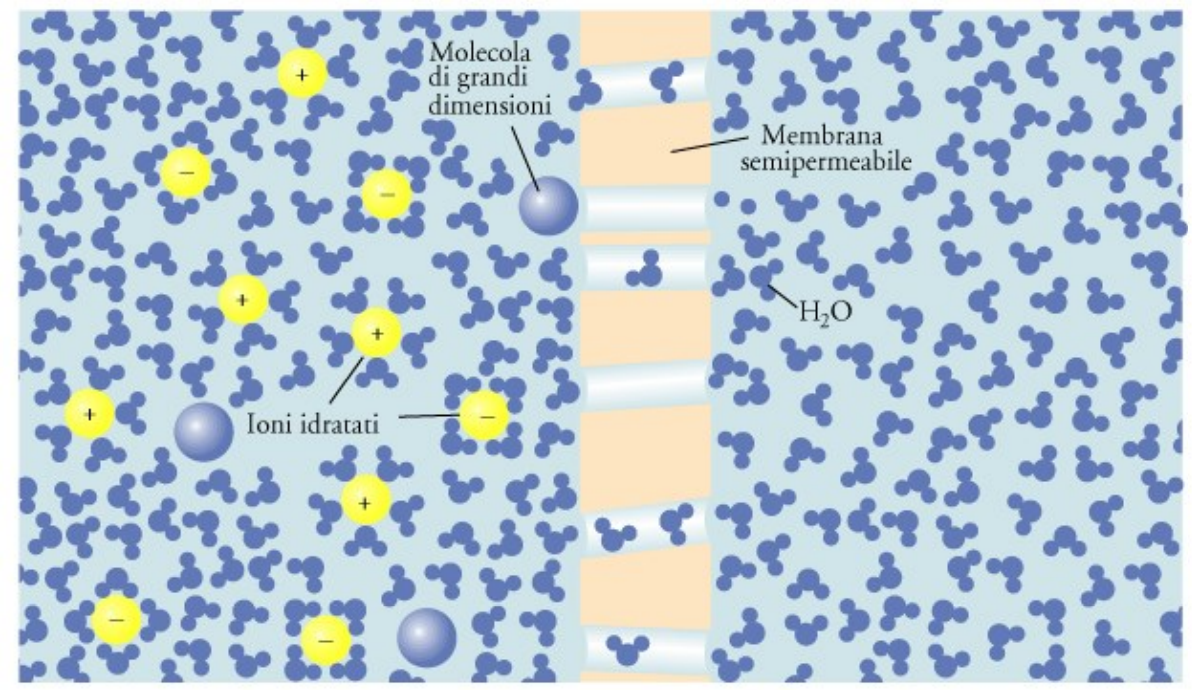
\includegraphics[width=10cm]{immagini/osmosi.png}
\end{figure}
\newpage
Gli ioni in acqua vengono circondati da molecole di H$_2$O, per cui lo ione non è una entità isolata in soluzioni, ma bensì si forma un aggregato molto più voluminoso dello ione stesso, sia per quello positivo che per quello negativo. Quindi lo ione non può passare perché nell'istante in cui viene solvatato diventa molto voluminoso, e siccome uno ione idratato è più voluminoso dei pori della membrana non riuscirà a passare, rimanendo confinato nella zona in cui l'abbiamo posto, mentre l'acqua sarà libera di spostarsi.

\hspace{0.5cm}\begin{minipage}{0.5\textwidth}
    \begin{figure}[H]
        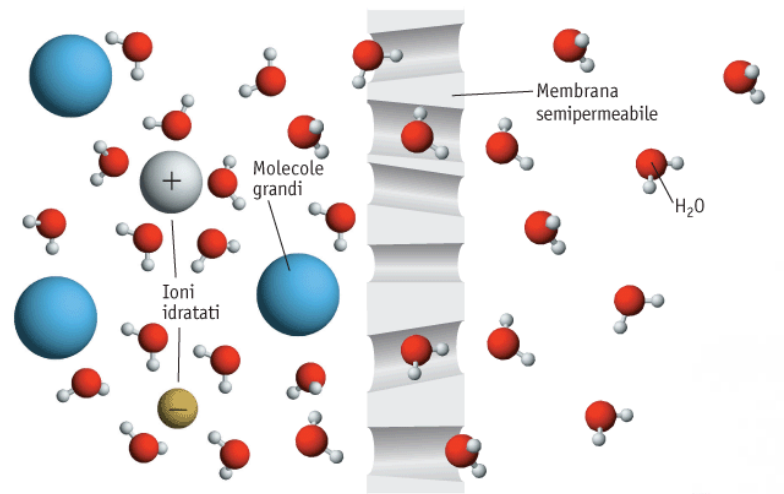
\includegraphics[width=6.5cm]{immagini/membrana.png}
    \end{figure}
\end{minipage}
\hspace{-1.3cm}\begin{minipage}{0.5\textwidth}
    \begin{figure}[H]
        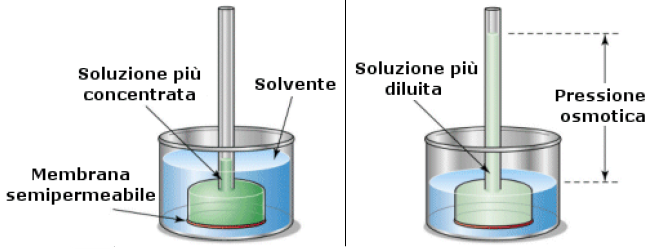
\includegraphics[width=8.5cm]{immagini/pressione_osmotica.png}
    \end{figure}
\end{minipage}

\vspace{0.3cm}Ci si è accorti che mettendo a contatto tramite una membrana o due soluzioni con concentrazioni diverse o una soluzione con del solvente, quello che succede nel tempo è un passaggio di solvente netto da un posto all'altro (anche se può spostarsi in entrambe le direzioni).

Immaginiamo di avere un recipiente separato in due parti con volume identico da una membrana semipermeabile. Supponiamo anche che ci sia una soluzione di H$_2$O e NaCl a sinistra e solo H$_2$O a destra, nel tempo noteremo un passaggio netto di solvente da destra verso sinistra, per cui nella soluzione avremo un aumento di volume significativo e parimenti una diminuzione del volume a destra.

Lo stesso effetto si avrebbe se a destra ci fosse, anziché solo solvente, una soluzione meno concentrata rispetto quella a sinistra.

Se il volume aumenta, sulla membrana si eserciterà una pressione (mentre prima, essendo i due volumi identici le pressioni esercitate sui due lati erano identiche e quindi la pressione totale era nulla) che porta la membrana a flettersi.
\subsubsection{Pressione osmotica}
Abbiamo visto che in una soluzione e un solvente a contatto tramite una membrana, il solvente tende ad andare nella soluzione. C'è quindi una tendenza a diluire quest'ultima, che è la forza motrice dell'osmosi: tutte le volte che mettiamo due soluzioni a contatto, la più diluita vedrà il suo solvente spostarsi verso la soluzione più concentrata, tendendo a eguagliare le concentrazioni laddove è possibile.

\E chiaro quindi che si può applicare una pressione esterna per bloccare il fenomeno.

Si definisce allora \textit{pressione osmotica} la pressione minima necessaria da applicare affinché l'osmosi non avvenga.

\begin{figure}[htp]
    \centering
    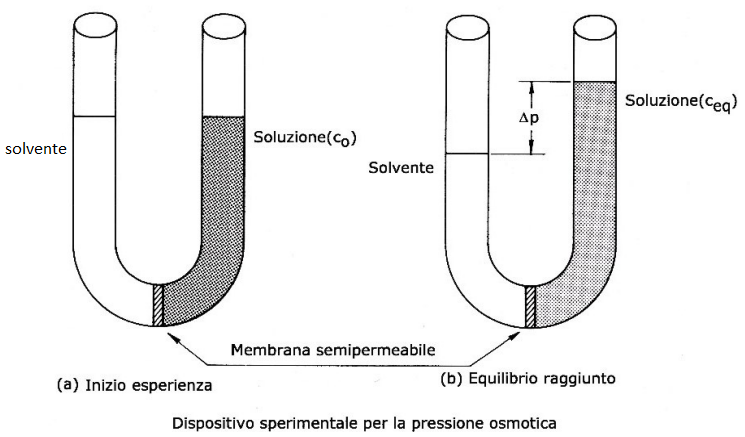
\includegraphics[width=11cm]{immagini/tubo_a_U.png}
\end{figure}

Un esempio classico è quello di un tubo a forma di U in cui è posta una membrana semipermeabile. Si riempie un braccio con solvente e l'altro con una soluzione di una data concentrazione (se avessimo avuto due soluzioni con concentrazioni diverse il discorso non sarebbe cambiato) in modo da avere volumi uguali. Ci si accorge, dopo che è passato un po' di tempo, che i volumi non sono più uguali: il livello del solvente è più basso, quindi una parte di questo si è spostato nell'altro braccio.

Il dislivello che si forma tra i due volumi esercita una pressione sulla membrana, la quale se flessibile si flette (se è un setto poroso non si flette, se è una membrana si).

Il risultato che si ottiene è una diluizione della soluzione.

\E chiaro che nell'istante in cui la membrana si flette perché si esercita una pressione, ci sarà una sorta di ostacolo per le molecole che cercano di passare dal solvente alla soluzione dato proprio dalla pressione che si oppone a questo movimento. Quindi il fenomeno dell'osmosi non va all'infinito, cioè non tutto il solvente va nella soluzione: ne passa tanto fino a quando la pressione $\Delta P$ non ne impedisce il passaggio ulteriore. A questo punto si raggiunge l'equilibrio.

La pressione $\Delta P$ esercitata dal dislivello è quella che chiamiamo pressione osmotica.

A seconda delle concentrazioni abbiamo:

\begin{itemize}
    \item Soluzione isotonica: la soluzione ha la stessa concentrazione dell'altra con cui è a contatto ;
    \item Soluzione ipertonica: la soluzione è più concentrata rispetto a quella con cui è a contatto;
    \item Soluzione ipotonica: la soluzione è meno concentrata rispetto a quella con cui è a contatto.
\end{itemize}

\subsubsection{ES. I globuli rossi}
La membrana esterna di un globulo rosso è una membrana semi-permeabile che scambia sia ioni che acqua con i liquidi delle cellule. Se si trova immerso in una soluzione avente la stessa concentrazione dei suoi liquidi interni, pressione interna e esterna sono uguali, per cui le soluzioni sono isotoniche e il globulo rosso ha la classica forma. Infatti quando si fa una flebo il contenuto deve avere una pressione osmotica analoga a quella del sangue.

Se invece la soluzione esterna è ipotonica, cioè povera di sali minerali, allora la soluzione interna sarà più concentrata. Da fuori allora l'acqua attraverserà la membrana del globulo, entrerà dentro e lo farà gonfiare potendo perfino farlo scoppiare (in questo caso si parla di emolisi).
 
Se invece la soluzione in cui è immerso è ipertonica, i liquidi al suo interno usciranno per diluire la soluzione esterna, facendo rinsecchire o persino implodere il globulo. Ciò può avvenire con un'alimentazione ricca di sale.

Ne segue che quando abbiamo la pressione alta c'è una soluzione ipertonica, quando abbiamo la pressione bassa una soluzione ipotonica.

Ecco perché non possiamo bere né l'acqua di mare né l'acqua distillata.

\begin{figure}[htp]
    \centering
    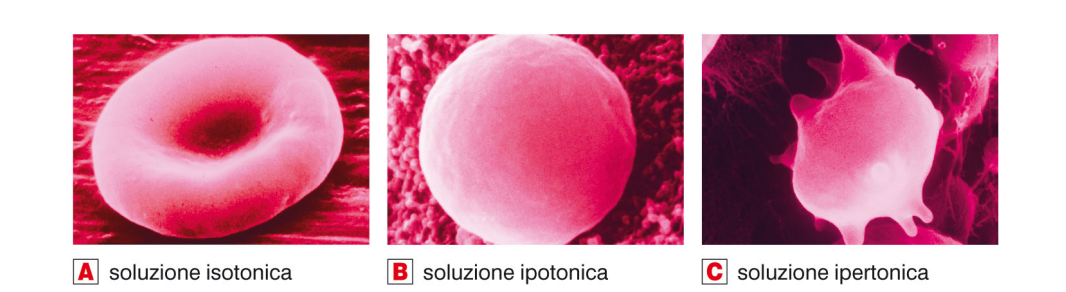
\includegraphics[width=14cm]{immagini/sangue.png}
\end{figure}

Calcoliamo adesso la pressione osmotica.
Si parte dalla legge dei gas, $PV=nRT$. Nel caso particolare della pressione osmotica sarà

$$\Pi V=nRT$$

Se dividiamo entrambi i membri per $V$, al secondo membro avremo $n/V$, che rappresenta la molarità (qui chiamata concentrazione $c$):

$$ \Pi = c R T i$$

Per quale motivo fisico l'acqua tende a diluire le sostanze più concentrate?

Abbiamo visto che l'acqua può attraversare, attraverso i pori, la membrana in entrambe le direzioni.

Consideriamo il caso della soluzione a sinistra e del solvente a destra. Da un punto di vista statistico a sinistra ci sono due eventi: se abbiamo messo esattamente lo stesso volume di solvente da un lato e di soluzione dall'altro, a sinistra avremo meno molecole di acqua perché a parità di volume una parte di questo sarà occupato dagli ioni. Questi ultimi inoltre sono diventati voluminosi e non riescono a passare, ma alcuni di questi insistono lo stesso sul poro della membrana e lo "otturano" parzialmente. Quindi mentre dal lato del solvente il 100\% dei pori è a disposizione delle molecole di H$_2$O, dal lato della soluzione no perché alcuni sono resi non disponibili per le molecole di acqua a sinistra.

Ne segue che, seppure l'acqua attraversi la membrana da entrambi i lati, il passaggio netto non è uguale a zero, cioè passano maggiormente molecole da destra verso sinistra, per cui a un certo punto avremo un accumulo di solvente da un lato fin quando la membrana si fletterà a tal punto da non permettere più un passaggio tale da far modificare il volume delle due soluzioni. L'equilibrio sarà comunque dinamico: le particelle passano ma non abbastanza da far cambiare volume.

\subsection{In sintesi: proprietà colligative}
\begin{enumerate}
    \item Tensione di vapore
    \item Innalzamento ebullioscopico
    \item Abbassamento crioscopico
    \item Pressione osmotica
\end{enumerate}
Sono dette colligative perché non dipendono solo dalla concentrazione, ma dal numero di particelle che si ha in soluzione. Tale dipendenza è rappresentata dal coefficiente $i$ di Van't Hoff, pari al numero di ioni in cui gli elettroliti si dissociano. Un \textbf{elettrolita} è una specie chimica che in soluzione si dissocia generando ioni.

Ma chi ci garantisce che ciò che mettiamo in soluzione si dissoci totalmente?

Per gli \textit{elettroliti forti} è ragionevole fare quest'assunzione, ma ci sono speci dette \textit{elettroliti deboli} per cui non è così. L'aggettivo forte sta per "totalmente dissociato", mentre debole sta per "parzialmente dissociato".

Quando abbiamo a che fare con elettroliti deboli (es. l'acido acetico) si parla di \textit{grado di dissociazione} $\alpha$, che è definito come il rapporto tra la quantità dissociata e quella iniziale:

$$\alpha=\frac{n_{dissociate}}{n_{iniziali}}$$

Chiaramente per gli elettroliti forti $\alpha=1$, ossia il numero di molecole dissociate è uguale al numero di molecole iniziali.

Il coefficiente di Van't Hoff va allora corretto così:

$$i=\big[1 + (\gamma - 1)\alpha \big]$$

dove $\gamma$ è il numero di particelle ottenute per effetto della dissociazione per unità formula (es. per NaCl $\gamma=2$).

\begin{center}
    \begin{tabular}{p{9cm}p{3.5cm}p{3.5cm}}
        & \hspace{1cm}$i$ per & \hspace{1cm}$i$ per\\
        Composto & soluzioni 1.00 M & soluzioni 0.100 M\\[0.5 ex]
        \hline\\[-0.4cm]
        Non elettroliti & 1.00 (ideale) & 1.00 (ideale)\\[0.5 ex]
        Saccarosio, C$_{12}$H$_{22}$O$_{11}$ & 1.00 & 1.00\\[0.5 ex]
        Se in soluzione ci sono 2 ioni per unità formula & 2.00 (ideale) & 2.00 (ideale)\\[0.5 ex]
        KBr & 1.77 & 1.88\\[0.5 ex]
        NaCl & 1.83 & 1.87\\[0.5 ex]
        Se in soluzione ci sono 3 ioni per unità formula & 3.00(ideale) & 3.00(ideale)\\[0.5 ex]
        K$_2$CO$_3$ & 2.39 & 2.45 \\[0.5 ex]
        K$_2$CrO$_4$ & 1.95 & 2.39\\[0.5 ex]
        Se in soluzione ci sono 4 ioni per unità formula & 4.00 (ideale) & 4.00 (ideale)\\[0.5 ex]
        K$_3$[Fe(CN)$_6$] & - & 2.85\\[0.5 ex]
    \end{tabular}
\end{center}

Sperimentalmente si nota che i valori di $i$ si discostano meno dall'idealità quando la soluzione è meno concentrata, cioè più diluita. Va da notare che una soluzione si può considerare ideale se è 10$^{-2}$ molare o più diluita, cioè la concentrazione massima è $0.01\;M$.